%%%%%%%%%%%%%%%%%%%%%%%%%%%%%%%%%%%%%%%%%%%%%%%%%%%%%%%%%%%%%%%%%%%%%%%%%%%%%%%%
%2345678901234567890123456789012345678901234567890123456789012345678901234567890
%        1         2         3         4         5         6         7         8

\documentclass[letterpaper, 10 pt, conference]{ieeeconf}  % Comment this line out if you need a4paper

%\documentclass[a4paper, 10pt, conference]{ieeeconf}      % Use this line for a4 paper

\IEEEoverridecommandlockouts                              % This command is only needed if 
                                                          % you want to use the \thanks command

\overrideIEEEmargins      

% Needed to meet printer requirements.
\usepackage{graphicx}
%In case you encounter the following error:
%Error 1010 The PDF file may be corrupt (unable to open PDF file) OR
%Error 1000 An error occurred while parsing a contents stream. Unable to analyze the PDF file.
%This is a known problem with pdfLaTeX conversion filter. The file cannot be opened with acrobat reader
%Please use one of the alternatives below to circumvent this error by uncommenting one or the other
%\pdfobjcompresslevel=0
%\pdfminorversion=4

% See the \addtolength command later in the file to balance the column lengths
% on the last page of the document

% The following packages can be found on http:\\www.ctan.org
%\usepackage{graphics} % for pdf, bitmapped graphics files
%\usepackage{epsfig} % for postscript graphics files
%\usepackage{mathptmx} % assumes new font selection scheme installed
%\usepackage{times} % assumes new font selection scheme installed
%\usepackage{amsmath} % assumes amsmath package installed
%\usepackage{amssymb}  % assumes amsmath package installed

\title{\LARGE \bf
Social Robots for Early Detection of Mental Heath Conditions
}


\author{Amrita Krishnaraj$^{1}$ and Chien-Ming Huang$^{2}$% <-this % stops a space
\thanks{*This work was not supported by any organization}% <-this % stops a space
\thanks{$^{1}$Amrita Krishnaraj Researcheris with the Laboratory of Computational sensing and Robotics,
        Johns Hopkins University, USA.
        {\tt\small akrishn9@jhu.edu}}%
\thanks{$^{2}$ Chien-Ming Huang is with Faculty of Computer science Engineering, Johns Hopkins University, USA.
        {\tt\small cmhuang@cs.jhu.edu}}%
}


\begin{document}



\maketitle
\thispagestyle{empty}
\pagestyle{empty}


%%%%%%%%%%%%%%%%%%%%%%%%%%%%%%%%%%%%%%%%%%%%%%%%%%%%%%%%%%%%%%%%%%%%%%%%%%%%%%%%
\begin{abstract}

Globally, mental health is a growing socio-economic burden and leads to negative ramifications including mortality and poor quality of life. Successful early detection of mental illness will make a significant, positive economic and societal impact. In an attempt to detect the early signs of depression, our research explores a social robot with 6 DOF and exhibits non-verbal behaviors. In this design, audio, video, and haptic inputs have been explored to detect user's emotional state. In addition, a pilot study has been conducted to study the interaction between the robot and participants, effectiveness of the robot, and response of the participants to the robot. These results can help inform the future design of social robots by illuminating details of one direction in early detection of mental conditions.

\end{abstract}


%%%%%%%%%%%%%%%%%%%%%%%%%%%%%%%%%%%%%%%%%%%%%%%%%%%%%%%%%%%%%%%%%%%%%%%%%%%%%%%%
\section{INTRODUCTION}

Mental health is a growing concern in both the developed and the developing countries. Around 1-in-6 people globally (15-20\%) have one or more mental illnesses \cite{}. In the United States, approximately 1 in 5 adults (46.6 million) experienced mental illness in 2017 \cite{} and over one-third (37\%) of students suffer from a mental health condition \cite{}. The financial burden associated with mental illness is substantial and costs America approximately \$193.2 billion per year \cite{}. Individuals living with serious mental illness face an increased risk of chronic medical conditions \cite{}, increased risk of suicide \cite{}, and involvement in anti-social activities \cite{}. Research has also shown prolonged hospitalization and delayed recovery due to negative psychological consequences throughout recovery.

Despite being critical to overall well-being and physical health, diagnoses and treatment of mental illnesses remain low \cite{}. Successful early identification of mental health conditions will make a significant, positive economic and societal impact. Emerging research indicates that intervening early can interrupt the negative course of some mental illnesses and may, in some cases, lessen long-term disability \cite{}. There has however been little research on early detection of mental conditions. 

The use of Social Assistive Robots(SARs) in mental health care is nascent, but represents a potentially useful tool in the professional's toolbox. Appealing characteristics of robots such as embodiment, tangibility and interactivity can be leveraged for early detection of mental conditions. In an attempt to leverage robot technology for the early detection of mental illnesses, we have explored the design space of social robots. Our research focuses on developing a social robot that perceives and interprets human emotional state and provides artificial emotion support. Affective touch is a crucial element of social bonding, and emotional support. It has received little research attention due to the technical and social difficult to study human touch. In our robot design, we have explored various haptic cues to provide artificial emotional support. The aim was to design and develop robots that will provide companionship and also collect information to detect early signs of mental illnesses. 

\section{ROBOT DESIGN}

The developed robot ''DOT'' can be seen in figure. The physical dimensions of the robot are 17x15x30 cms and weighs about 2.36 lbs. The robot has 6 DOF, eye-lids open and closing mechanism (2 DOF), eyeballs pan and tilt mechanism (2 DOF) and neck rotation similar to human head (2 DOF). The entire robot is covered with artificial fur to encourage the users to make physical contact with the robot. %The robot skeleton is composed of two main parts: the Head and the Thorax, both connected by a neck. The thorax houses the actuation mechanism for the neck movements and the controllers of the robot. The head houses the actuation mechanism and mechanics for the eyeballs and eye-lids motion.

\begin{figure}
\centering
    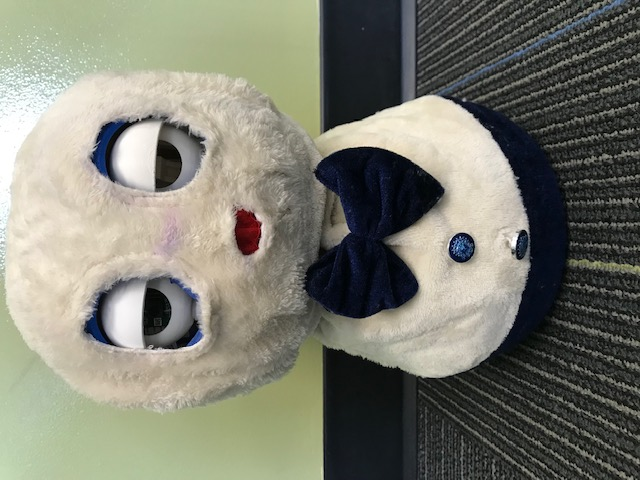
\includegraphics[width=6cm,height=4cm,angle=270]{IMG_8059.jpg}
\end{figure}



DOT has two layers to generate its proactive behavior: a behavior-planning layer and a behavior generation layer. Depending on its internal states DOT generates behavior. However, the internal state
of the robot is influenced by the users mood and emotions. The behaviour-planning layer takes input from the face tracking and emotion detection frameworks to generate the robot 's internal state. This layer then decides a particular response from a pool of predefined responses and sends basic behavioral
patterns to the behavior-generation layer. The behavior-generation layer generates control references for each actuator to perform the determined behavior. The behavior-generation layer adjusts parameters of priority of behaviors based on the internal states. This creates lifelike behavior that the user will be able to interpret.

\begin{figure}
\centering
    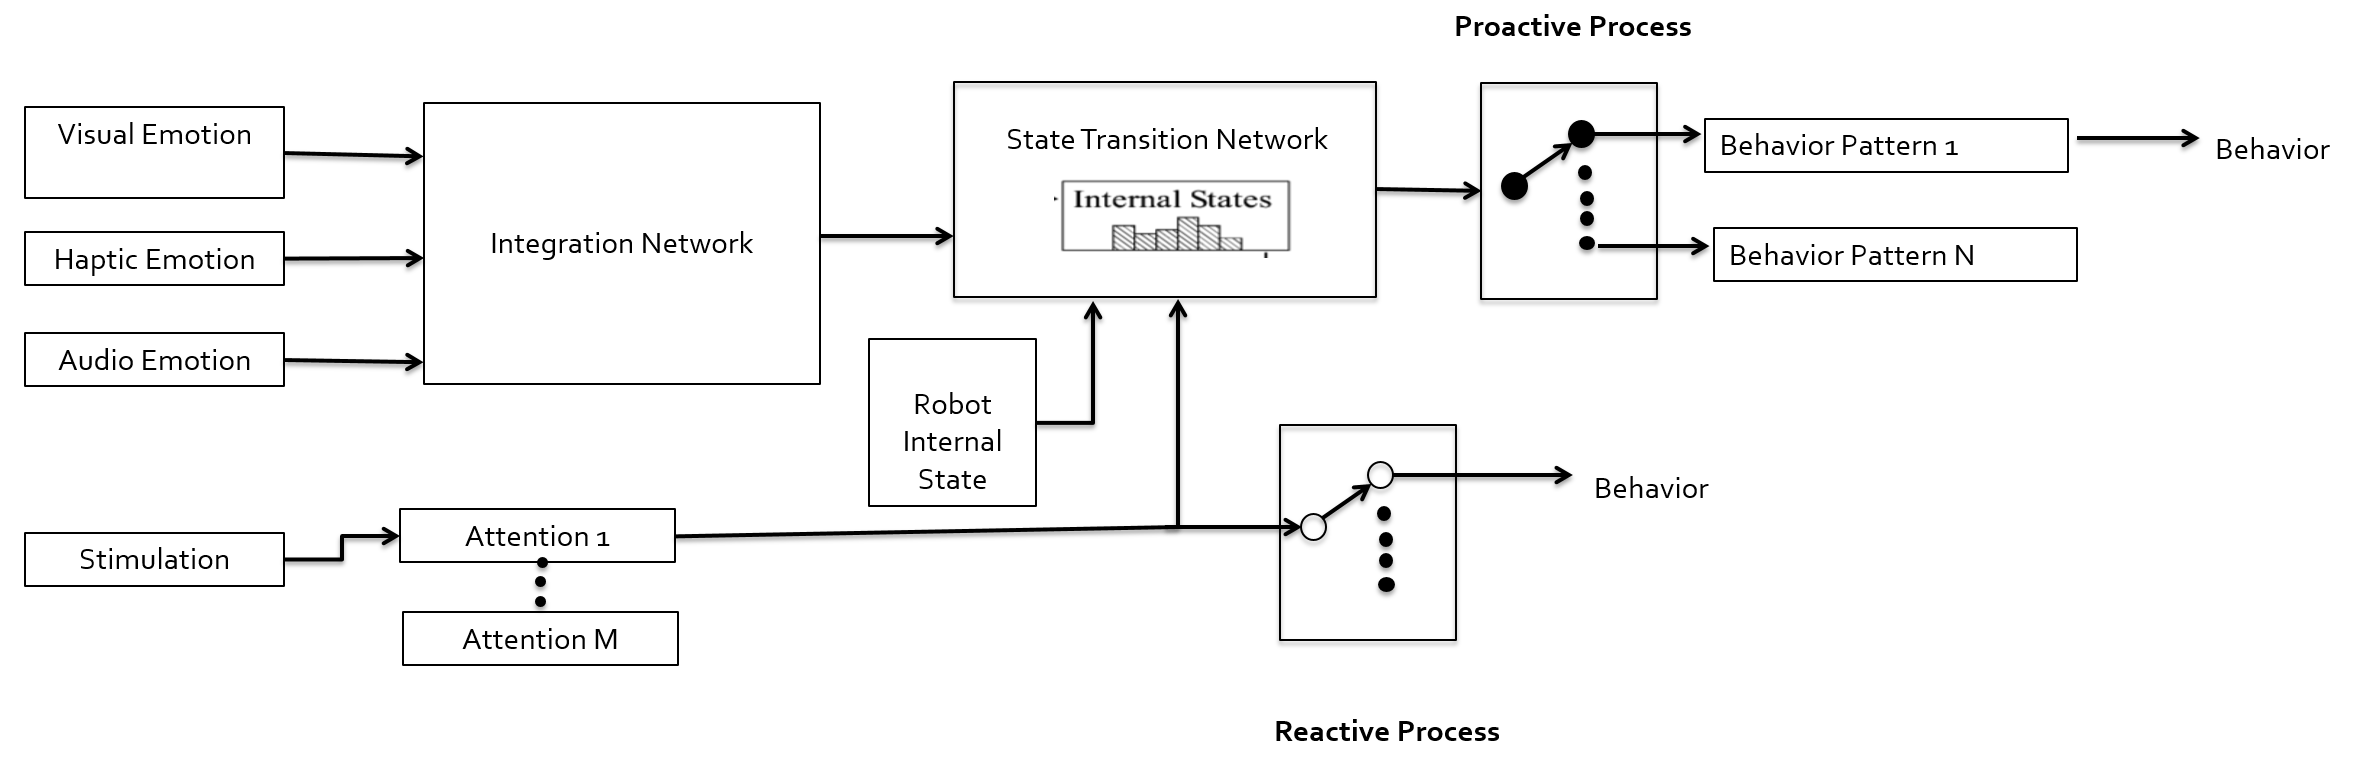
\includegraphics[width=9cm,height=4cm]{frame.png}
\end{figure}

\subsection{Haptic and Posture Cues}

A fabric tactile sensor, formed by sandwiching a resistive fabric between two conductive fabrics resulting in a matrix of $mxn$ contact points, is used for obtaining tactile information. Due to contact, the pressure increases and the pressure at each point is derived by measuring the potential difference across it. The contact regions in addition to previous contact history is used to classify the tactile input into one of the haptic gestures. The haptic gesture include Stroke, Contact, Hug, Hold, Rub, Pat, and Squeeze. The posture of the robot including toss, rock, and lift is achieved using the 6 DOF IMU. posture analysis is performed from the data received from the IMU to inform the robot about its surrounding and its position relative to the user.

\subsection{Face Tracking}
The face tracking module is designed to track the user across a room. The Single Short MultiBox detector(SSD) based on \cite{} is used for real-time detecting of faces. This detector is trained on both FER2013 \cite{} and IMDB \cite{} data sets and achieves an accuracy of 93\% in general object detection task together with real-time run-time performance (59FPS). In order to track the person across the room, the face position is maintained at the centre of the camera image plane. The difference is face position between successive images is considered as error and linear rotation is performed to maintain the face at the center of image using the control law.  Only the translation along the x and z axis is considered, a linear rotation at the neck is made to minimize the error vector.

\subsection{Emotion Classification Framework}

Emotion recognition module: 
The emotion recognition framework is implemented to take the sensor(camera, microphone, and tactile) inputs and interpret the emotional state of the robot. First, the audio signal is segmented and then the trained DNN network computes the emotion state distribution for each segment. The frames of video obtained from the camera is fed through the mini-Xception network to obtain the confusion matrix. The mini-Xception network is trained on FER-2013 data set and achieves 82.6\% accuracy. In order to synchronize the audio and video frames, a time stamp is attached to each video frame and audio segment and the average emotion of all the frames corresponding to an audio segment is used for prediction of emotion. Finally the two probabilities are combined using the Hidden Markov Model to obtain an emotional state with an accuracy of 92.3\%. 
\section{Experiments}
\subsection{Method}
To study the effectiveness of the robot, two participants, both female (M=23 yrs) who had not previously interacted with DOT were recruited from the local campus community through convenience sampling. The study took place in a controlled lab environment which was set like a home-theatre with a comfortable chair and side table.  
The subjects were first introduced to DOT. The experimenter pointed out some of the capabilities of the
robot(such as emotion recognition and face tracking) and indicated a list of haptic cues that the robot can interpret. During the study, artificial emotions were simulated in the participants. This
was achieved by the participant watching a video for 22 mins which was created using the ravdness \cite{} and International Affect Picture System \cite{} data-sets. The different emotions triggered were happiness, fear, sadness, anger, amusement, disgust and calmness. The participants were allowed to interact with the robot without any restrictions. After the task, a questionnaire was administered to the
subject followed by a short interview. 

\subsection{Measures}
The questionnaire covered several topics including the interactions between the subject and robot; and DOT’s actions and expressions. In order to objectively investigate the interaction of the participants with DOT, the activities of the participants during the study was recorded.

\section{RESULTS}
\textbf{Results of Video analysis -}
Analysis of the video recorded during the study showed that the participants continuous interaction between the subject and DOT. It was also observed that participants held the robot facing their point of observation for most parts of the experiment. Further, it was noted that the subjects turned the robot to face them at points when they wanted to talk to the robot or were checking on the robot. 

\textbf{Results of Questionnaire -}
Results of the questionnaire indicate that the participants liked the robot behavior and appearance. Questions concerning robot’s appearance and behavior (Eg. Was it comforting to hold the robot? Was the robots behavior disturbing? Was the robot too heavy/big to hold? ) was rated significantly high. The participants also showed strong intent to interact with the robot again.  

\textbf{Response of Participants to DOT -} The participants were excited to meet DOT and greeted it like a friend or a new person during the introduction. The participants interacted with DOT willingly from the beginning, speaking to it, stroking and hugging it. During the study, though they watched a video, the participants continuously
held the robot on their lap and kept stroking or patting.

\section{CONCLUSION}
SARs in general have been shown to be effective therapeutic assistants for intervention of mental illnesses. In our research work, we seek to explore the use of social robots for early detection of mental
illnesses. To this effect, a social robot was designed and a haptic based emotion recognition, gesture recognition and reactive responses were implemented. In investigating how to provide artificial emotional support, a proactive nonverbal behavior set has been developed and experimented though a pilot study. This work informs future research on the design of robots and motivates the integration of social robots for early detection of mental illnesses.

%\subsection{Selecting a Template (Heading 2)}

%First, confirm that you have the correct template for your paper size. This template has been tailored for output on the US-letter paper size. 
%It may be used for A4 paper size if the paper size setting is suitably modified.

%\subsection{Maintaining the Integrity of the Specifications}

%The template is used to format your paper and style the text. All margins, column widths, line spaces, and text fonts are prescribed; please do not alter them. You may note peculiarities. For example, the head margin in this template measures proportionately more than is customary. This measurement and others are deliberate, using specifications that anticipate your paper as one part of the entire proceedings, and not as an independent document. Please do not revise any of the current designations

%\section{MATH}

%Before you begin to format your paper, first write and save the content as a separate text file. Keep your text and graphic files separate until after the text has been formatted and styled. Do not use hard tabs, and limit use of hard returns to only one return at the end of a paragraph. Do not add any kind of pagination anywhere in the paper. Do not number text heads-the template will do that for you.

%Finally, complete content and organizational editing before formatting. Please take note of the following items when proofreading spelling and grammar:

%\subsection{Abbreviations and Acronyms} Define abbreviations and acronyms the first time they are used in the text, even after they have been defined in the abstract. Abbreviations such as IEEE, SI, MKS, CGS, sc, dc, and rms do not have to be defined. Do not use abbreviations in the title or heads unless they are unavoidable.

%\subsection{Units}

%\begin{itemize}

%\item Use either SI (MKS) or CGS as primary units. (SI units are encouraged.) English units may be used as secondary units (in parentheses). An exception would be the use of English units as identifiers in trade, such as Ò3.5-inch disk driveÓ.
%\item Avoid combining SI and CGS units, such as current in amperes and magnetic field in oersteds. This often leads to confusion because equations do not balance dimensionally. If you must use mixed units, clearly state the units for each quantity that you use in an equation.
%\item Do not mix complete spellings and abbreviations of units: ÒWb/m2Ó or Òwebers per square meterÓ, not Òwebers/m2Ó.  Spell out units when they appear in text: Ò. . . a few henriesÓ, not Ò. . . a few HÓ.
%\item Use a zero before decimal points: Ò0.25Ó, not Ò.25Ó. Use Òcm3Ó, not ÒccÓ. (bullet list)

%\end{itemize}


%\subsection{Equations}

%The equations are an exception to the prescribed specifications of this template. You will need to determine whether or not your equation should be typed using either the Times New Roman or the Symbol font (please no other font). To create multileveled equations, it may be necessary to treat the equation as a graphic and insert it into the text after your paper is styled. Number equations consecutively. Equation numbers, within parentheses, are to position flush right, as in (1), using a right tab stop. To make your equations more compact, you may use the solidus ( / ), the exp function, or appropriate exponents. Italicize Roman symbols for quantities and variables, but not Greek symbols. Use a long dash rather than a hyphen for a minus sign. Punctuate equations with commas or periods when they are part of a sentence, as in

%$$
%\alpha + \beta = \chi \eqno{(1)}
%$$

%Note that the equation is centered using a center tab stop. Be sure that the symbols in your equation have been defined before or immediately following the equation. Use Ò(1)Ó, not ÒEq. (1)Ó or Òequation (1)Ó, except at the beginning of a sentence: ÒEquation (1) is . . .Ó

%\subsection{Some Common Mistakes}
%\begin{itemize}


%\item The word ÒdataÓ is plural, not singular.
%\item The subscript for the permeability of vacuum ?0, and other common scientific constants, is zero with subscript formatting, not a lowercase letter ÒoÓ.
%\item In American English, commas, semi-/colons, periods, question and exclamation marks are located within quotation marks only when a complete thought or name is cited, such as a title or full quotation. When quotation marks are used, instead of a bold or italic typeface, to highlight a word or phrase, punctuation should appear outside of the quotation marks. A parenthetical phrase or statement at the end of a sentence is punctuated outside of the closing parenthesis (like this). (A parenthetical sentence is punctuated within the parentheses.)
%\item A graph within a graph is an ÒinsetÓ, not an ÒinsertÓ. The word alternatively is preferred to the word ÒalternatelyÓ (unless you really mean something that alternates).
%\item Do not use the word ÒessentiallyÓ to mean ÒapproximatelyÓ or ÒeffectivelyÓ.
%$\item In your paper title, if the words Òthat usesÓ can accurately replace the word ÒusingÓ, capitalize the ÒuÓ; if not, keep using lower-cased.
%\item Be aware of the different meanings of the homophones ÒaffectÓ and ÒeffectÓ, ÒcomplementÓ and ÒcomplimentÓ, ÒdiscreetÓ and ÒdiscreteÓ, ÒprincipalÓ and ÒprincipleÓ.
%\item Do not confuse ÒimplyÓ and ÒinferÓ.
%\item The prefix ÒnonÓ is not a word; it should be joined to the word it modifies, usually without a hyphen.
%\item There is no period after the ÒetÓ in the Latin abbreviation Òet al.Ó.
%\item The abbreviation Òi.e.Ó means Òthat isÓ, and the abbreviation Òe.g.Ó means Òfor exampleÓ.

%\end{itemize}


%\section{USING THE TEMPLATE}

%Use this sample document as your LaTeX source file to create your document. Save this file as {\bf root.tex}. You have to make sure to use the cls file that came with this distribution. If you use a different style file, you cannot expect to get required margins. Note also that when you are creating your out PDF file, the source file is only part of the equation. {\it Your \TeX\ $\rightarrow$ PDF filter determines the output file size. Even if you make all the specifications to output a letter file in the source - if your filter is set to produce A4, you will only get A4 output. }

%It is impossible to account for all possible situation, one would encounter using \TeX. If you are using multiple \TeX\ files you must make sure that the ``MAIN`` source file is called root.tex - this is particularly important if your conference is using PaperPlaza's built in \TeX\ to PDF conversion tool.

%\subsection{Headings, etc}

%Text heads organize the topics on a relational, hierarchical basis. For example, the paper title is the primary text head because all subsequent material relates and elaborates on this one topic. If there are two or more sub-topics, the next level head (uppercase Roman numerals) should be used and, conversely, if there are not at least two sub-topics, then no subheads should be introduced. Styles named ÒHeading 1Ó, ÒHeading 2Ó, ÒHeading 3Ó, and ÒHeading 4Ó are prescribed.

%\subsection{Figures and Tables}

%Positioning Figures and Tables: Place figures and tables at the top and bottom of columns. Avoid placing them in the middle of columns. Large figures and tables may span across both columns. Figure captions should be below the figures; table heads should appear above the tables. Insert figures and tables after they are cited in the text. Use the abbreviation ÒFig. 1Ó, even at the beginning of a sentence.





%   \begin{figure}[thpb]
%      \centering
%      \framebox{\parbox{3in}{We suggest that you use a text box to insert a graphic (which is ideally a 300 dpi TIFF or EPS file, with all fonts embedded) because, in an document, this method is somewhat more stable than directly inserting a picture.
%}}
      %\includegraphics[scale=1.0]{figurefile}
%      \caption{Inductance of oscillation winding on amorphous
       %magnetic core versus DC bias magnetic %field}
      %\label{figurelabel}
   %\end{figure}
   

%Figure Labels: Use 8 point Times New Roman for Figure labels. Use words rather than symbols or abbreviations when writing Figure axis labels to avoid confusing the reader. As an example, write the quantity ÒMagnetizationÓ, or ÒMagnetization, MÓ, not just ÒMÓ. If including units in the label, present them within parentheses. Do not label axes only with units. In the example, write ÒMagnetization (A/m)Ó or ÒMagnetization {A[m(1)]}Ó, not just ÒA/mÓ. Do not label axes with a ratio of quantities and units. For example, write ÒTemperature (K)Ó, not ÒTemperature/K.Ó

%\section{CONCLUSIONS}

%A conclusion section is not required. Although a conclusion may review the main points of the paper, do not replicate the abstract as the conclusion. A conclusion might elaborate on the importance of the work or suggest applications and extensions. 

%\addtolength{\textheight}{-12cm}   % This command serves to balance the column lengths
                                  % on the last page of the document manually. It shortens
                                  % the textheight of the last page by a suitable amount.
                                  % This command does not take effect until the next page
                                  % so it should come on the page before the last. Make
                                  % sure that you do not shorten the textheight too much.

%%%%%%%%%%%%%%%%%%%%%%%%%%%%%%%%%%%%%%%%%%%%%%%%%%%%%%%%%%%%%%%%%%%%%%%%%%%%%%%%



%%%%%%%%%%%%%%%%%%%%%%%%%%%%%%%%%%%%%%%%%%%%%%%%%%%%%%%%%%%%%%%%%%%%%%%%%%%%%%%%



%%%%%%%%%%%%%%%%%%%%%%%%%%%%%%%%%%%%%%%%%%%%%%%%%%%%%%%%%%%%%%%%%%%%%%%%%%%%%%%%
%\section*{APPENDIX}

%Appendixes should appear before the acknowledgment.

%\section*{ACKNOWLEDGMENT}

%The preferred spelling of the word ÒacknowledgmentÓ in America is without an ÒeÓ after the ÒgÓ. Avoid the stilted expression, ÒOne of us (R. B. G.) thanks . . .Ó  Instead, try ÒR. B. G. thanksÓ. Put sponsor acknowledgments in the unnumbered footnote on the first page.



%%%%%%%%%%%%%%%%%%%%%%%%%%%%%%%%%%%%%%%%%%%%%%%%%%%%%%%%%%%%%%%%%%%%%%%%%%%%%%%%

%References are important to the reader; therefore, each citation must be complete and correct. If at all possible, references should be commonly available publications.


\newpage
\begin{thebibliography}{99}

\bibitem{c1} G. O. Young, ÒSynthetic structure of industrial plastics (Book style with paper title and editor),Ó 	in Plastics, 2nd ed. vol. 3, J. Peters, Ed.  New York: McGraw-Hill, 1964, pp. 15Ð64.
\bibitem{c2} W.-K. Chen, Linear Networks and Systems (Book style).	Belmont, CA: Wadsworth, 1993, pp. 123Ð135.




\end{thebibliography}




\end{document}
